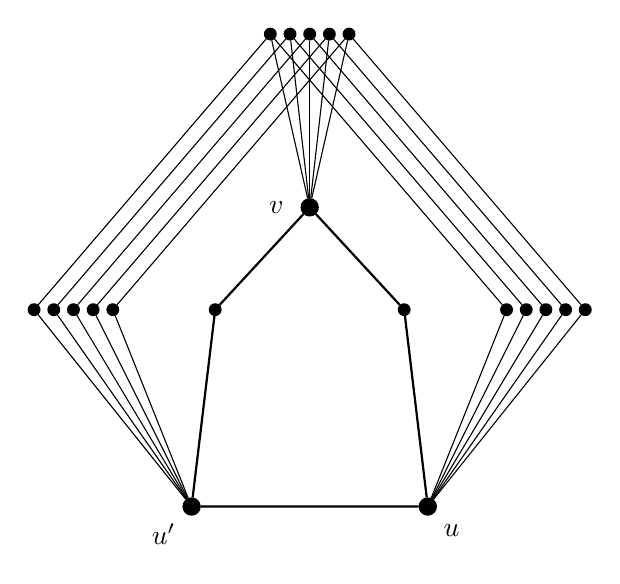
\begin{tikzpicture}[
        every node/.style={draw, circle, fill=black, inner sep=1.5pt},
        label distance=3pt, rotate=0
    ]
        % Glavna označena vozlišča (malo večja za poudarek)
        \node[inner sep=2.2pt, label=left:{$v$}] (v) at (0, 2.3) {};
        \node[inner sep=2.2pt, label=below left:{$u'$}] (u_prime) at (-1.5, -1.5) {};
        \node[inner sep=2.2pt, label=below right:{$u$}] (u) at (1.5, -1.5) {};

        % --- OSREDNJI C_5 ---
        % Stranski dve vozlišči, ki zapreta notranji petkotnik z v, u' in u
        \node (cL) at (-1.2, 1) {};
        \node (cR) at (1.2, 1) {};
        
        % Izris osrednjega petkotnika (debelejša linija)
        \draw[thick] (v) -- (cL) -- (u_prime) -- (u) -- (cR) -- (v);

        % --- PREOSTALI SNOP 5 POTI ---
        \foreach \i in {-2,-1,0,1,2} {
            % Izračun koordinat za enakomeren razmik zunanjih premic
            \coordinate (w\i) at ({0.25*\i}, 4.5);
            \coordinate (z\i) at ({-3.0 + 0.25*\i}, 1.0);
            \coordinate (zp\i) at ({3.0 + 0.25*\i}, 1.0);

            % Izris pik na vogalih zunanjih poti
            \node (wnode\i) at (w\i) {};
            \node (znode\i) at (z\i) {};
            \node (zpnode\i) at (zp\i) {};

            % Levi del: v -> vrh -> leva stran -> u'
            \draw (v) -- (wnode\i);
            \draw (wnode\i) -- (znode\i);
            \draw (znode\i) -- (u_prime);
            
            % Desni del: u -> desna stran -> vrh
            \draw (u) -- (zpnode\i);
            \draw (zpnode\i) -- (wnode\i);
        }
    \end{tikzpicture}